\documentclass[../main.tex]{subfiles}
\graphicspath{{figures/}{../figures/}}

\begin{document}
% \todo[color=green!40]{完成问题三模型的求解(sections/q3\_solution)}

由于问题5的变量较多,直接使用启发式搜索算法进行优化非常容易陷入局部最优解中,并且与实际最优解差距过大。因此,我们采用的优化策略是先逐个优化一个无人机对三个导弹的投放策略,再将得到的有效时间合并(去掉重复有效时间)。反复操作,得到多组不同的投放策略和有效时间,再对比这些投放策略,选取其中有效时间最长的一组作为最优投放策略。以下是核心步骤:

\noindent \textbf{步骤 1:设定初始参数与离散化时间轴}

首先定义导弹、无人机、烟幕弹及目标的物理参数,包括速度、加速度、尺寸等。同时设定仿真时间范围与步长,构建离散化时间轴,为后续动态模拟提供基础。

\noindent \textbf{步骤 2:建立目标模型与遮蔽判断机制} 

通过在真圆柱体上采样关键点,构建目标几何模型。利用辅助函数判断导弹视线是否被烟幕云团(球体)遮挡,即导弹-目标连线是否与烟幕球相交,作为有效遮蔽的核心判据。

\noindent \textbf{步骤 3:模拟烟幕弹投放与云团演化过程} 

根据无人机飞行方向、速度、投放时间及延迟起爆时间,计算每枚烟幕弹的投放点与爆炸点位置。结合重力与下沉速度,动态更新烟幕云团在空中的三维坐标随时间的变化,并判断其在有效生命周期内是否存在,形成时空分布的遮蔽区域。

\noindent \textbf{步骤 4:评估综合遮蔽效果与时间贡献} 

在整个时间轴上逐点判断各导弹是否被有效遮蔽。通过累计连续遮蔽区间,计算总有效遮蔽时间及各导弹的遮蔽时长。同时记录每架无人机单独作用时的贡献,用于分析协同效能。

\noindent \textbf{步骤 5:采用差分进化算法进行独立优化} 

对每架无人机的决策变量(方向角、速度、投放时序、延迟)进行独立优化。以最大化其单独贡献的遮蔽时间为目标函数,多次运行取最优解,确保搜索充分,避免陷入局部极值。

\noindent \textbf{步骤 6:结果整合分析与最优结果输出} 

将各无人机优化后的参数合并,评估整体协同遮蔽效果。

按照上式步骤,利用Pytho求解得到\textbf{最大有效时间为22.97s}.具体参数见表\ref{tab:...001}、表\ref{tab:....031}和表\ref{tab:....032}。

\begin{table}[H]
\caption{问题5投放策略-1}
\label{tab:...001} 
\centering
\begin{scriptsize}
\begin{tabular}{cccc}
\toprule[1.5pt]
无人机编号 & 烟幕干扰弹编号 & 无人机运动方向(度) & 无人机运动速度(m/s)  \\  
\midrule[1pt]
FY1        & 1              & 7.45               & 72.00                \\               
FY1        & 2              & 7.45               & 72.00                \\               
FY1        & 3              & 7.45               & 72.00                \\                
FY2        & 1              & 295.07             & 127.02               \\                
FY2        & 2              & 295.07             & 127.02               \\               
FY2        & 3              & 295.07             & 127.02               \\               
FY3        & 1              & 79.64              & 82.34                \\               
FY3        & 2              & 79.64              & 82.34                \\                
FY3        & 3              & 79.64              & 82.34                \\                
FY4        & 1              & 0                  & 70.00                \\                
FY4        & 2              & 0                  & 70.00                \\               
FY4        & 3              & 0                  & 70.00                \\               
FY5        & 1              & 120.32             & 104.78               \\               
FY5        & 2              & 120.32             & 104.78               \\                
FY5        & 3              & 120.32             & 104.78               \\               
\bottomrule[1.5pt]
\end{tabular}
\end{scriptsize}
\end{table}

\begin{table}[H]
\caption{问题5投放策略-2}
\label{tab:....031} 
\centering
\begin{scriptsize}
\begin{tabular}{cccc}
\toprule[1.5pt]
烟幕干扰弹投放点的x坐标 (m) & 烟幕干扰弹投放点的y坐标 (m) & 烟幕干扰弹投放点的z坐标 (m) & 烟幕干扰弹起爆点的x坐标 (m) \\
\midrule[1pt]
17800.00 & 0.00  & 1800.00 & 17800.00 \\  % FY1-烟幕弹#1
17871.39 & 9.33  & 1800.00 & 17903.52 \\  % FY1-烟幕弹#2
19121.47 & 172.77& 1800.00 & 19180.73 \\  % FY1-烟幕弹#3
12425.78 & 489.95& 1400.00 & 12458.62 \\  % FY2-烟幕弹#1
12707.30 & -111.76&1400.00 & 12851.56 \\  % FY2-烟幕弹#2
13363.47 & -1514.23&1400.00& 13757.49 \\  % FY2-烟幕弹#3
6502.06  & -253.36&700.00  & 6509.76  \\  % FY3-烟幕弹#1
6516.87  & -172.36&700.00  & 6555.07  \\  % FY3-烟幕弹#2
6531.68  & -91.36 &700.00  & 6564.69  \\  % FY3-烟幕弹#3
11064.40 & 2000.00&1800.00 & 11099.40 \\  % FY4-烟幕弹#1
11134.40 & 2000.00&1800.00 & 11228.20 \\  % FY4-烟幕弹#2
11204.40 & 2000.00&1800.00 & 11239.40 \\  % FY4-烟幕弹#3
12151.52 & -549.23&1300.00 & 12064.24 \\  % FY5-烟幕弹#1
12069.53 & -409.04&1300.00 & 11821.44 \\  % FY5-烟幕弹#2
11858.99 & -49.06 &1300.00 & 11759.02 \\  % FY5-烟幕弹#3
\bottomrule[1.5pt]
\end{tabular}
\end{scriptsize}
\end{table}

\begin{table}[H]
\caption{问题5投放策略-3(烟幕弹起爆点补充+有效遮蔽)}
\label{tab:....032} 
\centering
\begin{scriptsize}
\begin{tabular}{cccc}
\toprule[1.5pt]
烟幕干扰弹起爆点的y坐标 (m) & 烟幕干扰弹起爆点的z坐标 (m) & 有效干扰时长 (s) & 干扰的导弹编号 \\
\midrule[1pt]
0.00  & 1800.00 & 2.60 & M1 \\  % FY1-烟幕弹#1
13.53 & 1799.01 & 4.50 & M1 \\  % FY1-烟幕弹#2
180.51& 1796.62 & 0.00 & M3  \\  % FY1-烟幕弹#3
419.77& 1398.18 & 4.12 & M1 \\  % FY2-烟幕弹#1
-420.10&1364.81 & 3.38 & M2 \\  % FY2-烟幕弹#2
-2356.40&1137.45& 0.00 & M3  \\  % FY2-烟幕弹#3
-211.24& 698.68 & 1.75 & M1 \\  % FY3-烟幕弹#1
36.61  & 667.38 & 2.77 & M2 \\  % FY3-烟幕弹#2
89.26  & 675.63 & 0.00 & M3 \\  % FY3-烟幕弹#3
2000.00& 1798.78 & 0.00 & M1  \\  % FY4-烟幕弹#1
2000.00& 1791.20 & 0.00 & M2 \\  % FY4-烟幕弹#2
2000.00& 1798.78 & 0.00 & M3 \\  % FY4-烟幕弹#3
-399.99& 1286.66 & 1.04 & M1 \\  % FY5-烟幕弹#1
15.16  & 1192.22 & 3.51 & M2 \\  % FY5-烟幕弹#2
121.89 & 1282.50 & 0.00 & M3 \\  % FY5-烟幕弹#3
\bottomrule[1.5pt]
\end{tabular}
\end{scriptsize}
\end{table}

问题5部分结果可视化见图\ref{Figure_11111}和图\ref{Figure_12222}.

\begin{figure}[H]
\centering
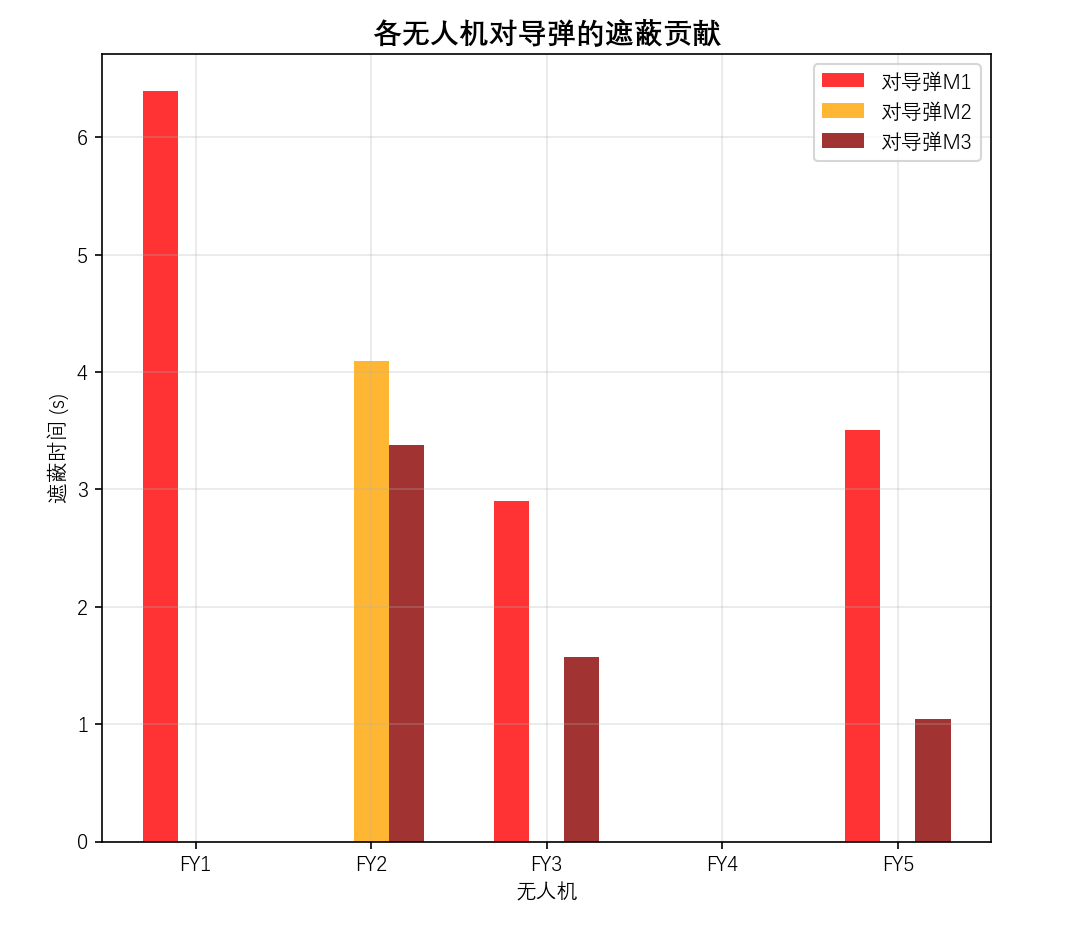
\includegraphics[scale=0.45]{问题五可视化图1.png}
\caption{各无人机对导弹的遮蔽贡献}
\label{Figure_11111}
\end{figure}

\begin{figure}[H]
\centering
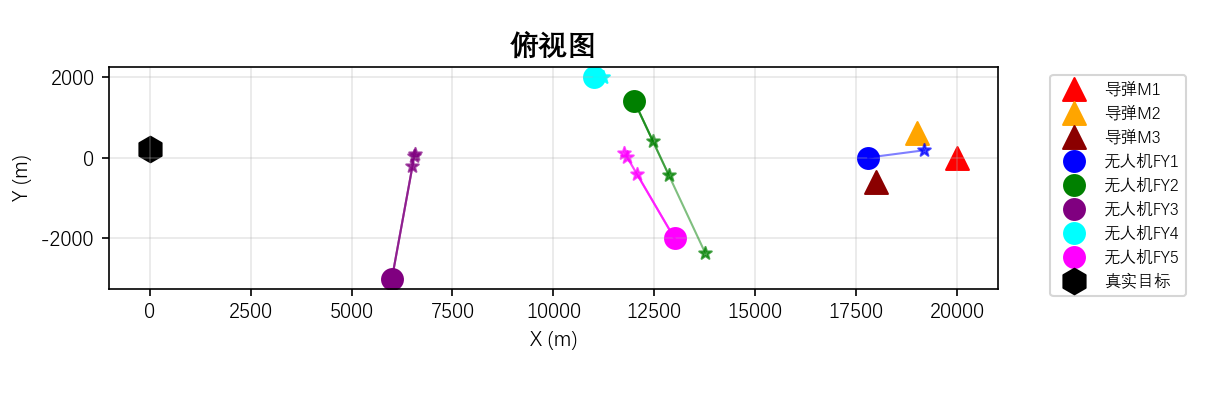
\includegraphics[scale=0.45]{问题5结果可视化2.png}
\caption{无人机、导弹和烟雾轨迹俯视图}
\label{Figure_12222}
\end{figure}



\end{document}